\section{COMPARISON OF CORRECTED UU AND CU TEST RESULTS 修正的UU和CU试验结果的比较}

\Paragraph{Results for Kawasaki and Lagunillas Clays: Kawasaki和Lagunillas黏土的结果:}

\begin{paracol}{2}
    
    Specific examples illustrating the application of the authors' methods of correcting UU and CU test data for sample disturbance will be presented first. In reiteration, the primary objective of the correction is to arrive at an undrained shear strength for triaxial compression of a specimen subjected to perfect sampling, that is, the specimen had a preshear effective stress equal to $\overline{\sigma}_{ps}$ (\autoref{equation:1}) and the in-situ void ratio. Test data for Kawasaki Clay I will be used for the illustrative examples.

    \switchcolumn

    首先将给出具体示例,这些示例说明作者针对样本干扰校正UU和CU试验数据的方法的应用。 重申一下,校正的主要目的是在经受完美采样的样品上获得不排水的剪切强度,以进行三轴压缩,也就是说,样品有一个预剪切有效应力等于$\overline{\sigma}_{ps}$(\cnequationref{equation:1})和原位空隙率。 Kawasaki黏土I的试验数据将用于说明示例。

    \switchcolumn*

    \emph{Correction of UU Data for Test $\overline{UU}-(18-5)-1$} (strain rate effects will be neglected).

    \switchcolumn

    \emph{对试验$\overline{UU}-(18-5)-1$的UU数据进行校正}(应变率影响将被忽略)。
  
    \switchcolumn*

    1. Measured data (\autoref{figure:6}): $S_u=0.46{\rm kg/cm^2}$ and $\overline{\sigma}_r=0.34{\rm kg/cm^2}$.

    2. Equivalent OCR (\autoref{figure:4}): Since specimen depth was 21.2 m, $\overline{\sigma}_{ps}=0.95{\rm kg/cm^2}$. Therefore, the equivalent ${\rm OCR}=\overline{\sigma}_{ps}/\overline{\sigma}_r=0.46/0.82=0.56{\rm kg/cm^2}$.

    3. Corrected strength: For an OCR=2.80, and using \autoref{figure:12}, $S_u~{\rm at}~\overline{\sigma}_c/S_u~{\rm at}~\overline{\sigma}_{cm}=0.82$. Since this ratio is also assumed equal to $S_u~{\rm at}~\overline{\sigma}_r/S_u~{\rm at}~\overline{\sigma}_{ps}$, the corrected $S_u=0.46/0.82=0.56{\rm kg/cm^2}$.

    \switchcolumn

    1.实测数据(\cnfigureref{figure:6}):$S_u=0.46{\rm kg/cm^2}$,$\overline{\sigma}_r=0.34{\rm kg/cm^2}$。
    
    2.等效OCR(\cnfigureref{figure:4}):由于样品深度为21.2 m,$\overline{\sigma}_{ps}=0.95{\rm kg/cm^2}$。因此,等效${\rm OCR}=\overline{\sigma}_{ps}/\overline{\sigma}_r=0.46/0.82=0.56{\rm kg/cm^2}$。
   
    3.校正强度:对于OCR=2.80,并使用\cnfigureref{figure:12},$S_u~{\rm at}~\overline{\sigma}_c/S_u~{\rm at}~\overline{\sigma}_{cm}=0.82$。 由于还假定该比率等于$S_u~{\rm at}~\overline{\sigma}_r/S_u~{\rm at}~\overline{\sigma}_{ps}$,因此校正后的$S_u=0.46/0.82=0.56{\rm kg/cm^2}$。

\end{paracol}

\Paragraph{Correction of CU Data for Depth of 23 M: CU数据深度为23米的修正:}

\begin{paracol}{2}

    \emph{1. Hvorslev parameters:} Values of the Hvorslev parameters are shown in \autoref{figure:15} for both the Lagunillas clay and Kawasaki Clay I where $\overline{\sigma}_e$, was based on values of $\Delta{e}/(1+e_0)$ in \autoref{figure:9} and \autoref{figure:10} rather than water content, which varied erratically. The parameters were determined on the basis of $\overline{CU}$ and \emph{CID} tests, although $\overline{UU}$ and $\overline{RCIU}$ test data have been added for interest.

    \switchcolumn

    \emph{1. Hvorslev参数:}Lagunillas黏土和Kawasaki黏土I的Hvorslev参数值如\cnfigureref{figure:15}所示,其中$\overline{\sigma}_e$是基于\cnfigureref{figure:9}和\cnfigureref{figure:10}中的$\Delta{e}/(1+e_0)$值,而不是水含量,这是不规则的变化。 尽管已添加了$\overline{UU}$和$\overline{RCIU}$试验数据,但这些参数是根据$\overline{CU}$和\emph{CID}试验确定的。

\end{paracol}

\begin{figure}[!htbp]
    \centering
    \subfigure[Kawasaki Clays I]{
        \label{figure:15a}
        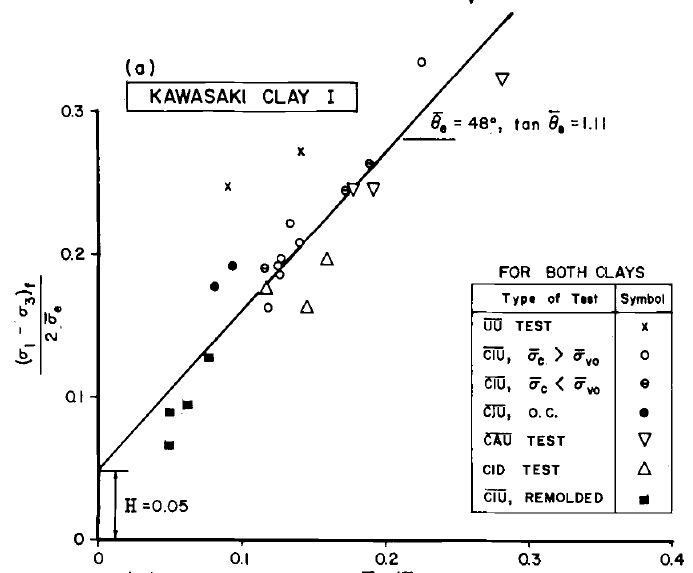
\includegraphics[width=0.48\textwidth]{figures/figure-15a.png}
    }
    \subfigure[Lagunilla Clay]{
        \label{figure:15b}
        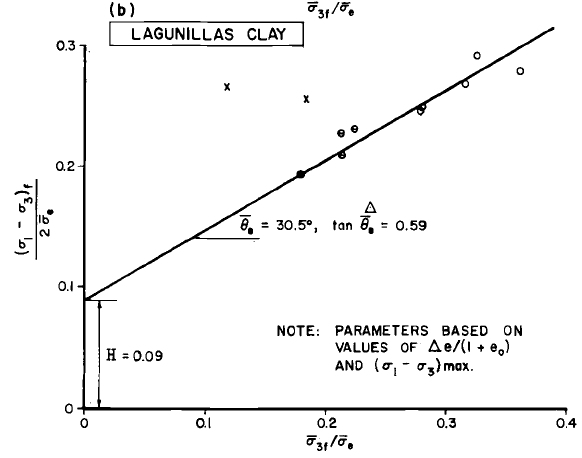
\includegraphics[width=0.48\textwidth]{figures/figure-15b.png}
    }
    \caption{Hvorslev Parameters.}
    \addtocounter{figure}{-1}
    \vspace{-5pt}
    \renewcommand{\figurename}{图}
    \caption{Hvorslev参数}
    \renewcommand{\figurename}{Figure}
    \label{figure:15}
\end{figure}
\begin{sidewaystable}[p]
    \centering
    \footnotesize
    \caption{COMPARISON OF CORRECTED UNDRAINED STRENGTH FROM UU AND CU TESTS ON NORMALLY CONSOLIDATED KAWASAKI AND LAGUNILLAS CLAYS.}
    \addtocounter{table}{-1}
    \vspace{-8pt}
    \renewcommand{\tablename}{表}
    \caption{正常固结的Kawasaki和Lagunillas黏土上UU和CU试验的修正不排水强度的比较。}
    \vspace{4pt}
    \renewcommand{\tablename}{Table}
    \begin{threeparttable}
    \setlength{\tabcolsep}{1.0mm}{
        \begin{tabular}{llllllllllllllll}
            \toprule
            \multirow{3}{*}{Location}        & \multirow{3}{*}{Clay} & \multirowcell{3}[1pt][l]{Depth,\\m} & \multirowcell{3}[1pt][l]{$\overline{\sigma}_{v0}$,\\$\rm{kg/cm^2}$} & \multirowcell{3}[1pt][l]{$\overline{\sigma}_{ps}$,\\$\rm{kg/cm^2}$} & \multicolumn{2}{l}{\multirowcell{2}[1pt][l]{$S_u/\overline{\sigma}_{v0}$ From \\UU Tests}} & \multicolumn{4}{l}{$S_u/\overline{\sigma}_{v0}$ From CIU Tests}                          & \multicolumn{2}{l}{\multirowcell{2}[1pt][l]{Measured\tnote{c}\\$\frac{S_u(UU)}{S_u(CIU)}$}} & \multicolumn{2}{l}{\multirowcell{2}[1pt][l]{Corrected\tnote{d}\\$\frac{S_u(UU)}{S_u(CIU)}$}} & \multirowcell{3}[1pt][l]{$\frac{S_u(UU)}{S_u(CIU)}$\tnote{e}\\$S_u(CU)$ from\\$CA-\overline{UU}$ Tests\\(11)} \\
                                             &                       &                          &                        &                        & \multicolumn{2}{l}{}                                 & \multicolumn{2}{l}{Measured\tnote{a}} & \multicolumn{2}{l}{Corrected\tnote{b}} & \multicolumn{2}{l}{}                          & \multicolumn{2}{l}{}                           &                     \\
                                             &                       &                          &                        &                        & \makecell[l]{Measured\\(1)}                 & \makecell[l]{Corrected\tnote{f}\\(2)}                 & \makecell[l]{$\overline{\sigma}_c=\overline{\sigma}_{v0}$\\(3)}             & \makecell[l]{$\overline{\sigma}_c=\overline{\sigma}_{ps}$\\(4)}            & \makecell[l]{$\overline{\sigma}_c=\overline{\sigma}_{v0}$\\(5)}             & \makecell[l]{$\overline{\sigma}_c=\overline{\sigma}_{ps}$\\(6)}             & \makecell[l]{$\overline{\sigma}_c=\overline{\sigma}_{v0}$\\(7)}                     & \makecell[l]{$\overline{\sigma}_c=\overline{\sigma}_{ps}$\\(8)}                     & \makecell[l]{$\overline{\sigma}_c=\overline{\sigma}_{v0}$\\(9)}                      & \makecell[l]{$\overline{\sigma}_c=\overline{\sigma}_{ps}$\\(10)}                     &                     \\
            \midrule
            \multirowcell{2}[1pt][l]{Kawasaki, \\~~Japan} & \multirowcell{2}[11pt][l]{Clay I,P.I.=31$\%$\\Clay I,P.I.=36$\%$\\Clay II,P.I.=43$\%$} &  \makecell[l]{20.5\\25\\36}                        & \makecell[l]{1.60\\1.88\\2.62}                       & \makecell[l]{0.92\\1.08\\1.64}                       & \makecell[l]{0.31\tnote{g}\\0.26\tnote{g}\\0.27\tnote{g}}                         & \makecell[l]{0.38\\0.32\\0.33}                          & \makecell[l]{0.485\\0.45\\0.475}              & \makecell[l]{0.42\\0.37\\0.36}             & \makecell[l]{0.43\\0.395\\0.42}              & \makecell[l]{0.40\\0.35\\0.335}              & \makecell[l]{0.64\\0.58\\0.57}                      & \makecell[l]{0.74\\0.70\\0.75}                      & \makecell[l]{0.88\\0.81\\0.78}                       & \makecell[l]{0.95\\0.91\\0.98}                      & \makecell[l]{1.12\\0.89\\1.00}                    \\
                                             &                       & \multicolumn{9}{l}{Average}                                                                                                                                                                      &  0.59                     & 0.73                      & 0.82                       & 0.95                      & 1.00                    \\
            \makecell[l]{Lagunillas, \\~~Venezuela}            & \makecell[l]{plastic clay,\\~~~~P.I.=37$\%$}   & 6.4                         & 0.62                       & \makecell[l]{0.40\\(Estimated)}                       & 0.255\tnote{h}                         & 0.345                          & 0.40              & 0.335             & 0.38              & 0.325              & 0.64                      & 0.77                      &  0.91                      & 1.05                      & $\cdots$                    \\
            \bottomrule
        \end{tabular}}%
        \begin{tablenotes}
            \item[a] From \autoref{figure:7} and \autoref{figure:8} or similar data. $\overline{\sigma}_c=\overline{\sigma}_{v0}$ means that $S_u$ is taken at $\overline{\sigma}_c=\overline{\sigma}_{v0}$; for $\overline{\sigma}_c=\overline{\sigma}_{ps}$, $S_u$ is taken at $\overline{\sigma}_c=\overline{\sigma}_{v0}$. 来自\cnfigureref{figure:7}和\cnfigureref{figure:8}或类似数据。$\overline{\sigma}_c=\overline{\sigma}_{v0}$代表$S_u$在$\overline{\sigma}_c=\overline{\sigma}_{v0}$时获得,$\overline{\sigma}_c=\overline{\sigma}_{ps}$代表$S_u$在$\overline{\sigma}_c=\overline{\sigma}_{ps}$时获得。
            \item[b] Based on Hvorslev parameters. That is, $\Delta{S_u}=H\Delta{\overline{\sigma}_e}$. 基于Hvorslev参数,即$\Delta{S_u}=H\Delta{\overline{\sigma}_e}$。
            \item[c] Columns (1) over (3) and (1) over (4) respectively. 分别对应于列1/列3和列1/列4。
            \item[d] Columns (2) over (5) and (2) over (6) respectively. 分别对应于列2/列5和列2/列6。
            \item[e] $S_u(CU)$ from $S_u/\overline{\sigma}_{1c}$ ratio from $CA-\overline{UU}$ tests at $\overline{\sigma}_{1c}$ values 2-4 times $s_u/\overline{\sigma}_{v0}$ from Column 2. 来自$CA-\overline{UU}$试验的$S_u/\overline{\sigma}_{1c}$的$S_u(CU)$在数值上时列2中$s_u/\overline{\sigma}_{v0}$的2-4倍。
            \item[f] Correction for Kawasaki based on taking O.C.R. = 2.85 ($\overline{\sigma}_r/\overline{\sigma}_{ps}=0.35$ which corresponds to values for the better samples). Correction for Lagunillas based on taking O.C.R. = 2.8 ($\overline{\sigma}_r/\overline{\sigma}_{ps}=0.36$). 根据O.C.R. = 2.85对Kawasaki的修正($\overline{\sigma}_r/\overline{\sigma}_{ps}=0.35$,对应于较好样本的值)。 根据O.C.R.修正Lagunillas  = 2.8($\overline{\sigma}_r/\overline{\sigma}_{ps}=0.35$)。
            \item[g] Average from UU and top one-third of U tests corrected to $t_f$ = 5 hr. UU和U试验的前三分之一的平均值已校正为$t_f$ = 5小时。
            \item[h] Average from UU tests for which ~r measurements available. 如果$\overline{\sigma}_r$可测量时UU试验的平均值。
        \end{tablenotes}
    \end{threeparttable}
    \label{table:4}%
\end{sidewaystable}


\begin{paracol}{2}
    
    \emph{2. Measured data:} For a depth of 23m \autoref{figure:4} shows that $\overline{\sigma}_{v0}=1.75{\rm kg/cm^2}$ and $\overline{\sigma}_{ps}=1.00{\rm kg/cm^2}$. From \autoref{figure:8} at $\overline{\sigma}_c=\overline{\sigma}_{ps}=1.00{\rm kg/cm^2}$, the measured $S_u=0.68{\rm kg/cm^2}$. For $\overline{\sigma}_c=1.00{\rm kg/cm^2}$, a representative value of $\Delta{e}/(1+e_0)=0.04$ from \autoref{figure:10}.

    \switchcolumn

    \emph{2.测量数据:}对于23m的深度,\cnfigureref{figure:4}表明$\overline{\sigma}_{v0}=1.75{\rm kg/cm^2}$,$\overline{\sigma}_{ps}=1.00{\rm kg/cm^2}$。\cnfigureref{figure:8}的$\overline{\sigma}_c=\overline{\sigma}_{ps}=1.00{\rm kg/cm^2}$,实测值$S_u=0.68{\rm kg/cm^2}$。 对于$\overline{\sigma}_c=1.00{\rm kg/cm^2}$,\cnfigureref{figure:10}的代表值$\Delta{e}/(1+e_0)=0.04$。

    \switchcolumn*

   \emph{3. Equivalent consolidation pressures} (\autoref{figure:10}): For $\Delta{e}/(1+e_0)=0.04$, $\overline{\sigma}_e=2.60{\rm kg/cm^2}$; this represents isotropic consolidation of a lab specimen to $\overline{\sigma}_c=\overline{\sigma}_{ps}=1.00{\rm kg/cm^2}$. For perfect sampling, $\Delta{e}/(1+e_0)=0$ and $\overline{\sigma}_e=\overline{\sigma}_{v0}=1.75{\rm kg/cm^2}$.

    \switchcolumn

    \emph{3.当量固结压力}(\cnfigureref{figure:10}):对于$\Delta{e}/(1+e_0)=0.04$,$\overline{\sigma}_e=2.60{\rm kg/cm^2}$;这表示实验室样品的各向同性固结至$\overline{\sigma}_c=\overline{\sigma}_{ps}=1.00{\rm kg/cm^2}$。 对于完美采样,$\Delta{e}/(1+e_0)=0$且$\overline{\sigma}_e=\overline{\sigma}_{v0}=1.75{\rm kg/cm^2}$。

    \switchcolumn*

    \emph{4. Corrected strength}: From \autoref{equation:2} if $\Delta{\overline{\sigma}_{3f}}=0$, $\Delta{S_u}=H\Delta{\overline{\sigma}_e}$; H = 0.05 from \autoref{figure:15} and $\Delta{\overline{\sigma}_e}=(1.75-2.60)=-0.85{\rm kg/cm^2}$ from above. Therefore the correction to $S_u$ for the volume change = $0.05\times{-0.85}=-0.043$, and the corrected $S_u=0.68-0.043\approx{0.64}{\rm kg/cm^2}$.

    \switchcolumn

    \emph{4.校正强度}:由\cnequationref{equation:2}可知,如果$\Delta{\overline{\sigma}_{3f}}=0$,则有$\Delta{S_u}=H\Delta{\overline{\sigma}_e}$;由\cnfigureref{figure:15}可得H = 0.05和从上面可得$\Delta{\overline{\sigma}_e}=(1.75-2.60)=-0.85{\rm kg/cm^2}$。 因此,对体积变化的$S_u$校正值为$0.05\times{-0.85}=-0.043$,校正后的$S_u=0.68-0.043\approx{0.64}{\rm kg/cm^2}$。

\end{paracol}

\begin{paracol}{2}

    \autoref{table:4} presents the comparison of $S_u$ from UU and CU tests as measured and after correction for the Kawasaki and Lagunillas clays. Columns 1 and 2 show the effect on $S_u$ of treating $\overline{\sigma}_{ps}/\overline{\sigma}_r$ as an OCR for the UU-type tests; the strength was increased by $28\pm{6}$ percent. Columns 3 through 6 present the effects of correcting for the volume decrease upon reconsolidation based on Hvorslev parameters at consolidation pressures of both $\overline{\sigma}_{ps}$ and $\overline{\sigma}_r$; the strength was decreased by 5 to 12 percent. Columns 7 through 10 present ratios of measured and corrected $S_u$ from UU tests to that from CIU tests based on the data in Columns 1 through 6. The effect of performing the authors' second method of correcting CU data for volume decreases is shown in Column 11.

    \switchcolumn

    \cntableref{table:4}列出了对Kawasaki和Lagunillas黏土进行测量和校正后的UU和CU试验中$S_u$的比较。 第1栏和第2栏显示了将$\overline{\sigma}_{ps}/\overline{\sigma}_r$作为UU型试验的OCR处理对$S_u$的影响; 强度提高了$28\pm{6}\%$。 第3列至第6列表示在固结压力均为$\overline{\sigma}_{ps}$和$\overline{\sigma}_r$时,基于Hvorslev参数校正固结时体积减小的效果。 强度降低了$5\%$至$12\%$。 第7到10列根据第1到6列的数据显示了UU试验与CIU试验的$S_u$校正比率。列11中显示了执行作者针对体积减少而校正CU数据的第二种方法的效果。

    \switchcolumn*

    Columns 10 and 11 are of greatest interest. If the analyses proposed by the authors were entirely correct, the ratios in these columns should have equalled unity since (1) The UU strength data had been adjusted to make $\overline{\sigma}_r=\overline{\sigma}_{ps}$,, and The CU strength data had been adjusted to make $\overline{\sigma}_c=\overline{\sigma}_{ps}$ and $\Delta{e}/(1+e_0)=0$ by two methods.

    \switchcolumn

    第10栏和第11栏最为重要。 如果作者提出的分析是完全正确的,则这些列中的比率应等于1,因为(1)已对UU强度数据进行了调整,使$\overline{\sigma}_r=\overline{\sigma}_{ps}$,并且(2)通过两种方法将CU强度数据调整为$\overline{\sigma}_c=\overline{\sigma}_{ps}$和$\Delta{e}/(1+e_0)=0$。
    
    \switchcolumn*
    
    That is, all of the data had been adjusted, in theory, to conditions corresponding to perfect sampling. The actual values in these columns varied from unity by a maximum of only 12 percent, which is considered good agreement in view of the large differences (Column 8 shows 23 to 30 percent) in strengths before corrections. However, these methods require further investigation to establish their limitations.

    \switchcolumn

    也就是说,从理论上讲,所有数据都已调整为与完美采样相对应的条件。 这些栏中的实际值最大相差只有12$\%$,鉴于校正前的强度差异很大(第8栏显示232$\%$至302$\%$),这被认为是很好的一致性。 但是,这些方法需要进一步研究以确定其局限性。

    \switchcolumn*

    As previously pointed out, there should not be agreement between $S_u$ from UU tests and that from CIU tests with $\overline{\sigma}_c=\overline{\sigma}_{v0}$ even for perfect samples, since $\overline{\sigma}_c$ will be less than $\overline{\sigma}_{v0}$ for normally consolidated clays. This is illustrated by the data in Column 9 where the ratio was only 0.85 4- 0.06.

    \switchcolumn
   
    如前所述,即使对于完美的样品,UU试验的$S_u$与$\overline{\sigma}_c=\overline{\sigma}_{v0}$条件下CIU试验得到的$S_u$也不应达成共识,因为对于正常固结的黏土,$\overline{\sigma}_c$会小于$\overline{\sigma}_{v0}$。 列9中的数据说明了这一点,该比率仅为$0.85\pm{0.06}$。
\end{paracol}